\section{Funzionamento dei test}
Questa sezione è dedicata al funzionamento e all'implementazione dei test presenti nell'applicazione. Per test si intende una procedura di misurazione che utilizza il sensore e il display, non si tratta di unit test. Tutto il codice discusso in questa sezione è parte del package \texttt{com.dosse.openldat.tests}.

In generale, un test utilizza una backend grafica per visualizzare qualcosa sul display mentre cattura i dati dal dispositivo, dopodiché analizza i dati raccolti per estrarre informazioni di interesse.

La principale difficoltà che l'analisi deve saper affrontare è la presenza di rumore sul segnale, e in particolar modo la presenza di retroilluminazione PWM. Il problema è gestito diversamente in ogni test, a seconda dell'informazione che si desidera estrarre, ma in generale si assume che in presenza di retroilluminazione PWM, il segnale di interesse è moltiplicato per un altro segnale di frequenza più alta (come se fosse una modulazione AM) e potenzialmente potrebbe avere anche un offset DC variabile.\\
I grafici in figura \ref{fig:pwm_example} mostrano come potrebbe presentarsi un segnale catturato dal sensore in presenza di PWM rispetto al segnale reale. Display diversi tipicamente hanno forme molto diverse per questo segnale.
\begin{figure}[H]
	\centering
	\begin{tikzpicture}
		\begin{axis}[name=Segnale, xmin=0,xmax=0.2,ymin=0,ymax=1023,width=.45\textwidth,xlabel=Tempo (s),ylabel=Valore,xticklabel style={/pgf/number format/fixed}]
			\addplot[black] file{Chapter04/res/pwm_example_desired.txt};
		\end{axis}
	\end{tikzpicture}
	\begin{tikzpicture}
		\begin{axis}[name=Segnale, xmin=0,xmax=0.2,ymin=0,ymax=1023,width=.45\textwidth,xlabel=Tempo (s),ylabel=Valore,xticklabel style={/pgf/number format/fixed}]
			\addplot[black] file{Chapter04/res/pwm_example_captured.txt};
		\end{axis}
	\end{tikzpicture}
	\caption{Segnale reale (sinistra) e possibile segnale catturato in presenza di retroilluminazione PWM (destra). (Simulato, non è una cattura reale)}
	\label{fig:pwm_example}
\end{figure}

In generale, si può dire che in presenza di retroilluminazione PWM, il segnale originale è ricostruibile osservando i picchi alti del segnale catturato, ma è importante ricordare che la presenza di questo tipo di disturbo impedisce di ricostruire accuratamente il segnale originale, soprattutto se ha componenti ad alta frequenza, e che ci sono momenti in cui la retroilluminazione del display è completamente spenta. Per questo motivo, la presenza di PWM influisce negativamente sull'accuratezza di tutti i test.\\
Indipendentemente dal tipo di retroilluminazione, comunque, è sempre bene impostare la luminosità del display al massimo e disattivare qualsiasi tipo di miglioramento dell'immagine prima di eseguire qualsiasi test, così da avere risultati più veritieri. Se la retroilluminazione varia di intensità durante i test, questi potrebbero produrre risultati non validi.

\subsection{Backend grafiche}
Il package \texttt{com.dosse.openldat.tests.testscreen} mette a disposizione due backend grafiche con cui i test possono disegnare sul display: una che utilizza OpenGL (\texttt{TestScreenGL}) e una che utilizza Swing (\texttt{TestScreenSwing}). La backend OpenGL ha più funzionalità ed è più rappresentativa del comportamento di un'applicazione grafica come un videogioco, mentre la backend Swing è più basilare ed è usata come fallback su sistemi che non supportano OpenGL, ma è più rappresentativa del comportamento di un'interfaccia grafica che di un gioco. La GUI comunque permette di scegliere tra le due backend, se lo si desidera.

L'immagine in figura \ref{fig:testscreen_example} mostra un esempio di output di una backend grafica.

\begin{figure}[h]
	\centering
	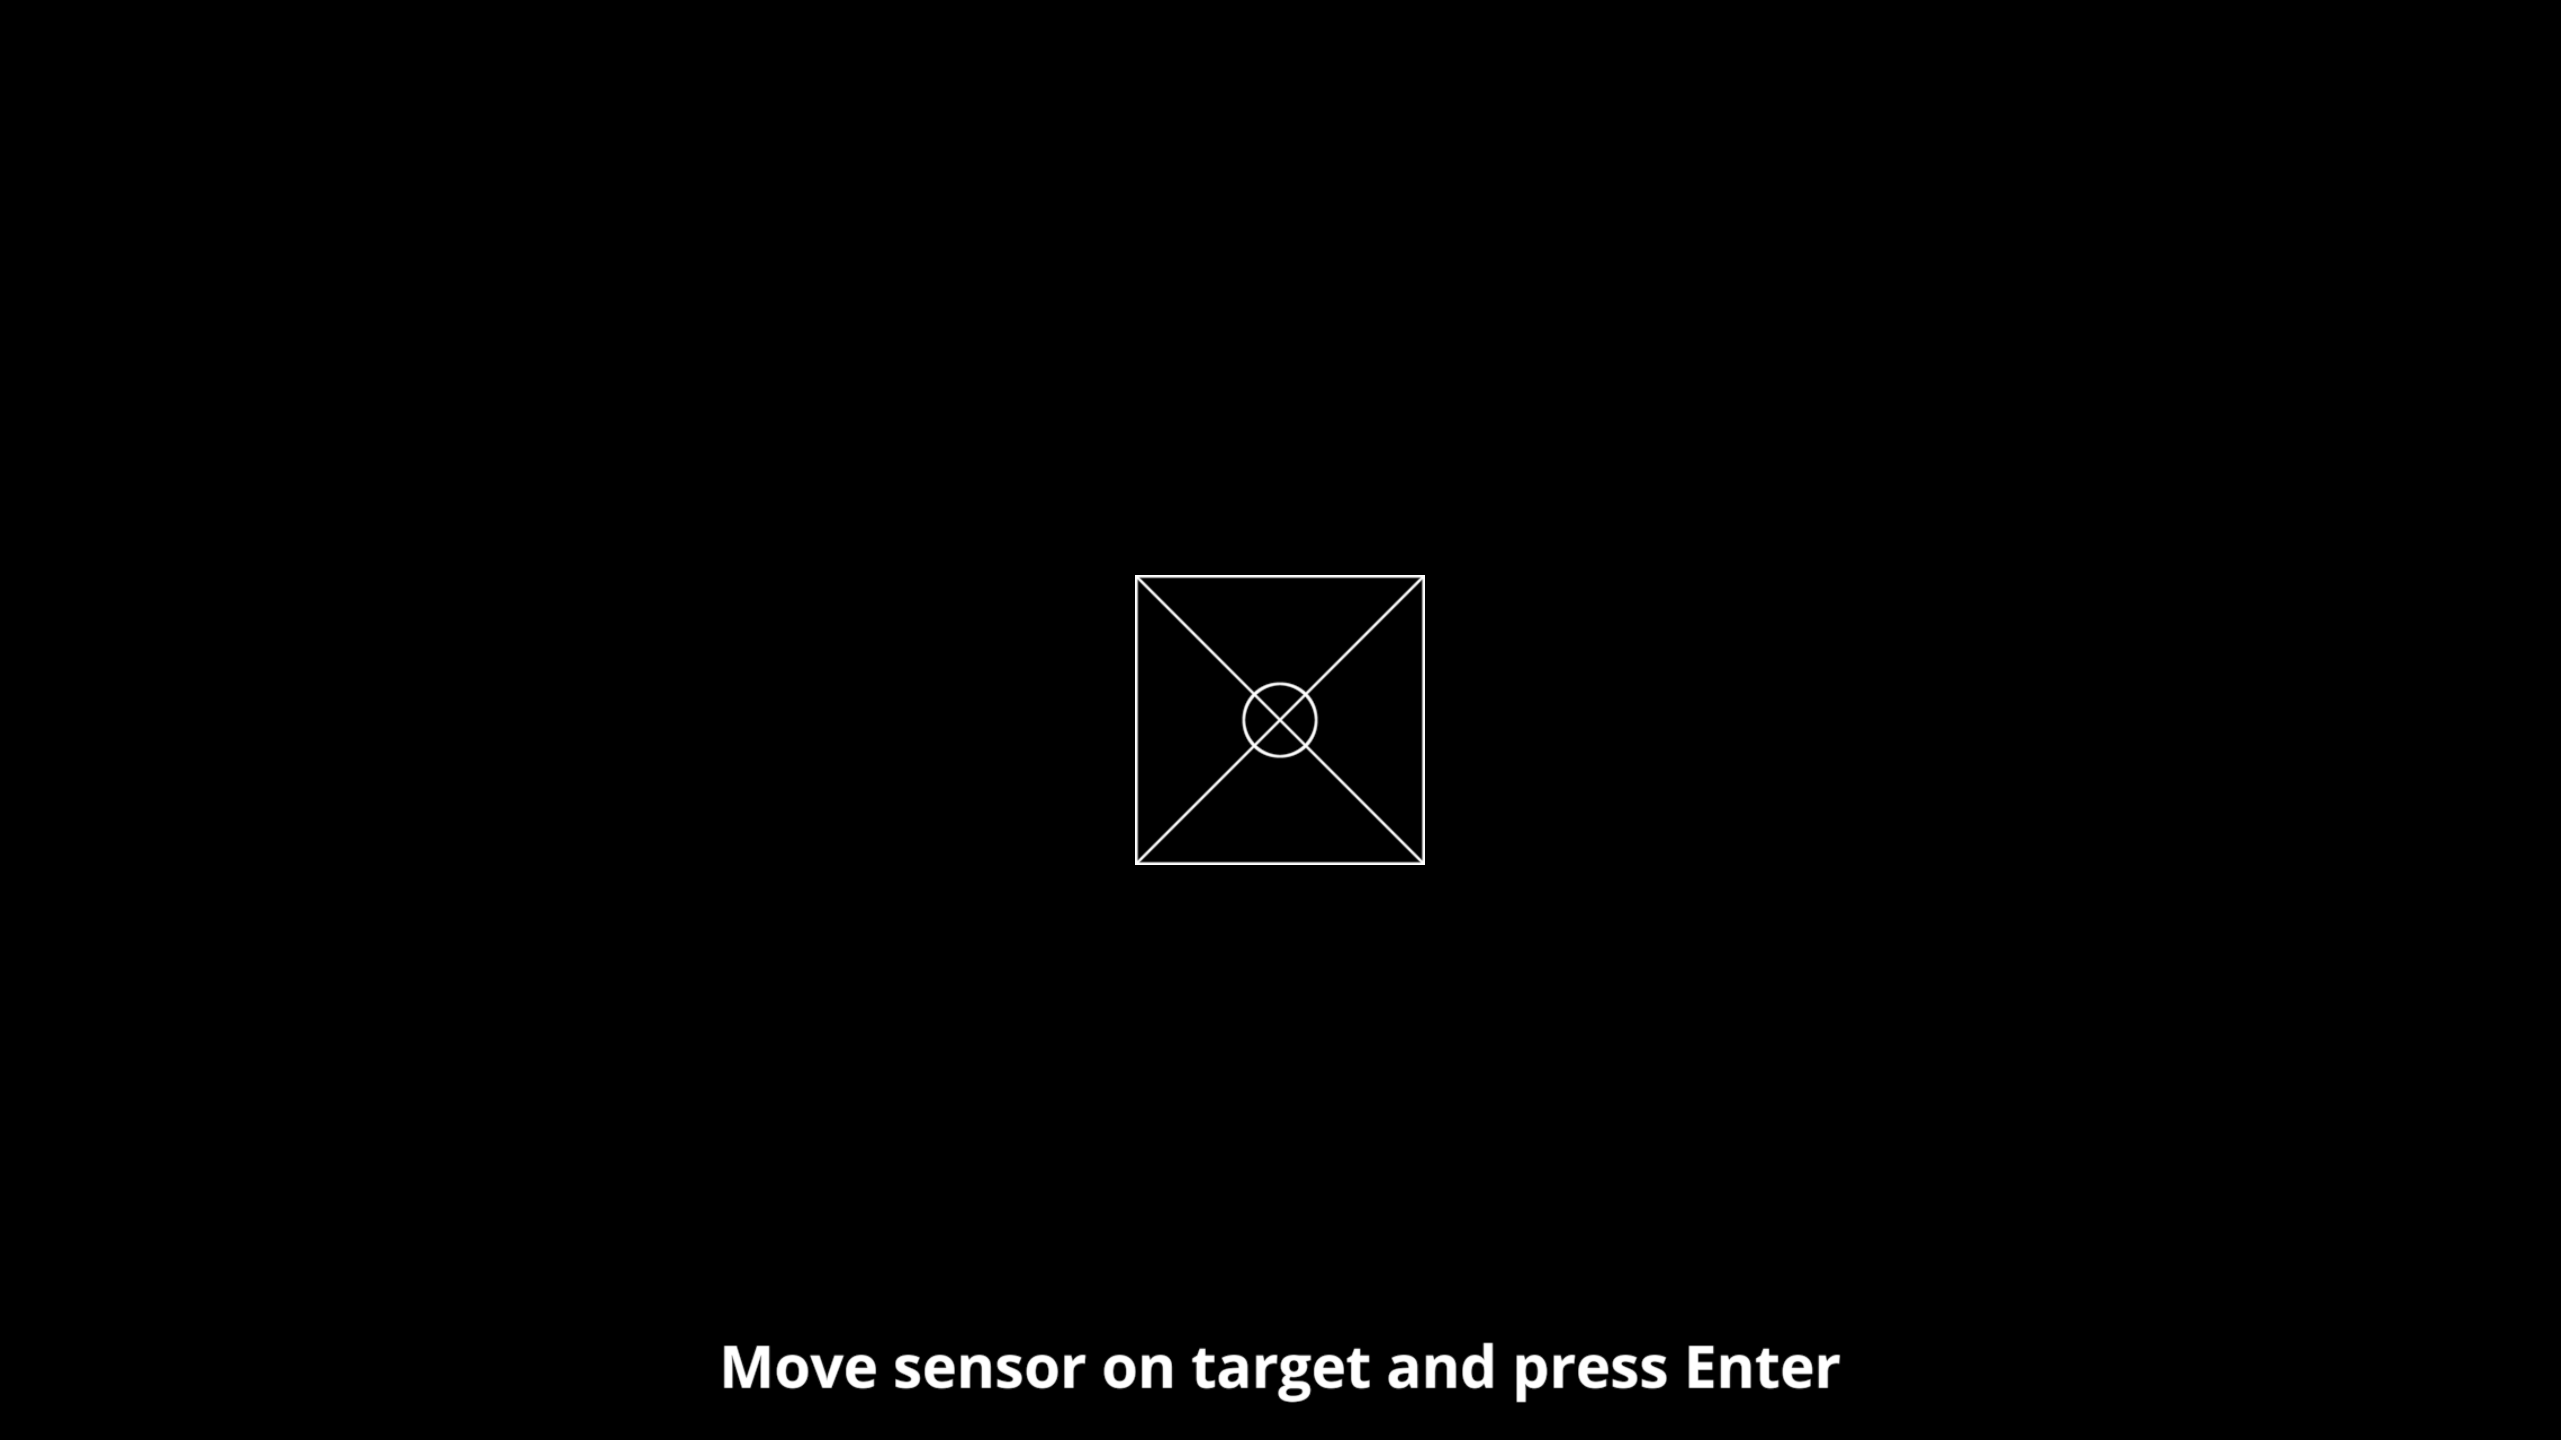
\includegraphics[width=\textwidth]{Chapter04/res/testscreen_example.png}
	\caption{Esempio di output di una schermata di test}
	\label{fig:testscreen_example}
\end{figure}

Entrambe le backend implementano un'interfaccia generica \texttt{ITestScreen}, che definsice le funzionalità minime che un backend deve avere e permette ai test di cambiare backend senza modifiche al codice. L'interfaccia definisce i seguenti metodi pubblici:
\begin{itemize}
	\item \texttt{public int getScreenW()}: ritorna la larghezza dello schermo in pixel
	\item \texttt{public int getScreenH()}: ritorna l'altezza dello schermo in pixel
	\item \texttt{public int getRefreshRate()}: ritorna il refresh rate dello schermo in Hz
	\item \texttt{public boolean setColor(float r, float g, float b)}: imposta il colore dello sfondo con tre valori RGB tra 0 e 1. Ritorna true se il colore nuovo è diverso da quello corrente, altrimenti false
	\item \texttt{public void setTarget(float x, float y, float size, boolean black)}: mostra il target e la scritta "Move sensor on target and press Enter" alle coordinate specificate. Le coordinate \texttt{x},\texttt{y} si riferiscono al centro del target e vanno tra 0 e 1, dove 0,0 è l'angolo in alto a sinistra e 1,1 è l'angolo in basso a destra. Impostando \texttt{black} a true, il target e il testo saranno di colore nero, altrimenti saranno bianchi. La dimensione del target è definita come $size*min(W,H)$. Un valore tipico per \texttt{size} è 0.15. Il target è sempre quadrato
	\item \texttt{public void setTargetAbsolute(float x, float y, float size, boolean black)}: analogo a \texttt{setTarget} ma le coordinate sono assolute anziché nel range 0-1
	\item \texttt{public void hideTarget()}: nasconde il target e la scritta precedentemente attivati con \texttt{setTarget} o \texttt{setTargetAbsolute}
	\item \texttt{public void setFlashOnClick(boolean flashOnClick)}: se impostato a \texttt{true}, quando l'applicazione riceve un click genera un flash bianco di 100ms
	\item \texttt{public boolean getFlashOnClick()}: ritorna \texttt{true} se è attualmente attivo il flash in risposta al click (default: disattivato)
	\item \texttt{public void flashColor(float r, float g, float b, double ms)}: genera un flash del colore specificato dai tre valori RGB tra 0 e 1 e della durata specificata
	\item \texttt{public void setFlicker(boolean bkFlicker)}: se impostato a \texttt{true}, il colore dello sfondo si alterna ad ogni fotogramma tra il colore impostato con \texttt{setColor} e il nero
	\item \texttt{public boolean isFlickering()}: ritorna \texttt{true} se è attualmente attivato il flickering (default: disattivato)
	\item \texttt{public void setFakeLoad(long cpuMs, long gpuMs)}: attiva la simulazione di un falso carico sulla CPU e sulla GPU (in millisecondi per frame). Non supportato dalla backend Swing
	\item \texttt{public long getFakeCPULoad()}: ritorna il falso carico attualmente simulato sulla CPU (default: 0)
	\item \texttt{public long getFakeGPULoad()}: ritorna il falso carico attualmente simulato sulla GPU (default: 0)
	\item \texttt{public void close()}: chuiude la schermata di test
	\item \texttt{public void onEnterPressed()}: callback che viene chiamato quando viene premuto il tasto Invio. I test fanno l'override di questo metodo per aggiungere il proprio codice di risposta all'evento. Se non viene fatto l'override, l'evento viene ignorato
	\item \texttt{public void onCancel()}: callback che viene chiamato se viene premuto il tasto Esc per annullare il test. I test fanno l'override di questo metodo per aggiungere il proprio codice di risposta all'evento. Se non viene fatto l'override, l'evento viene ignorato
	\item \texttt{public void onError(Exception e)}: callback che viene chiamato se si verificano errori irreversibili, per esempio in seguito a un crash del driver video. I test fanno l'override di questo metodo per aggiungere il proprio codice di risposta all'evento. Se non viene fatto l'override, il comportamento di default è stampare l'eccezione con il relativo stacktrace e terminare l'applicazione
\end{itemize}

Le due backend hanno due costruttori leggermente diversi:
\begin{itemize}
	\item \texttt{public TestScreenGL(int vsyncMode)}: inizializza la backend OpenGL 2.0 sullo schermo principale. È possibile specificare una modalità per il VSync tra le seguenti costanti definite nella classe stessa:
	\begin{itemize}
		\item \texttt{VSYNC\_OFF}: disabilita il VSync, consentendo le massime prestazioni e il minor ritardo possibile
		\item \texttt{VSYNC\_ON}: attiva il VSync classico con doppio buffering
		\item \texttt{VSYNC\_ON\_ALT}: utilizza il VSync fornito dal compositor del desktop, consentendo all'applicazione di funzionare come se il VSync fosse disattivato (quindi a framerate illimitato) ma evitando comunque il tearing. Non è supportato da tutte le combinazioni hardware e software
	\end{itemize}
	\item \texttt{public TestScreenSwing()}: inizializza la backend Swing sullo schermo principale. Non ci sono impostazioni per questa backend; il VSync (se presente) è fornito dal sistema e non è sotto il controllo dell'applicazione
\end{itemize}

Una volta inizializzata, la backend grafica continua l'esecuzione su un thread parallelo, lasciando al thread principale il compito di coordinare il test interagendo con la backend e con il driver del dispositivo.

Prima di proseguire, è necessario puntualizzare alcune caratteristiche delle backend grafiche:\begin{itemize}
	\item Entrambe le backend vengono eseguite in fullscreen borderless, non in fullscreen esclusivo. Su GNU/Linux, viene disattivato il compositor mentre il test è in esecuzione per evitare che questo penalizzi le performance
	\item La backend OpenGL utilizza lo stesso formato dei pixel e la stessa risoluzione del desktop, tuttavia, a causa di un bug nella libreria LWJGL 3.2.3, l'applicazione potrebbe non dichiarare il supporto HDR/WCG su Windows e quindi mostrare colori errati su display HDR. Questo problema è noto agli sviluppatori di LWJGL e sarà corretto nella release 3.3.0
	\item La backend Swing, poiché utilizza un toolkit grafico pensato per creare interfacce grafiche e non videogiochi, non ha modo di sincronizzarsi con il display, per cui funzioni come \texttt{setFlicker} potrebbero generare un microstuttering che non sarebbe normalmente presente in altre applicazioni grafiche
\end{itemize}

\subsection{Interfaccia standard dei test}
I test implementano tutti un'interfaccia comune, \texttt{ITest}, che definisce alcuni metodi che tutti i test devono implementare:
\begin{itemize}
	\item \texttt{public void begin()}: inizia l'esecuzione del codice del test. A seconda del test, questo può significare l'inizio effettivo del test o semplicemente un'operazione come chiedere all'utente di posizionare il sensore
	\item \texttt{public void cancel()}: richiede al test di terminare il prima possibile. A seconda di come è implementato il test, questo potrebbe terminare immediatamente o richiedere del tempo
	\item \texttt{public void onDone(Map results)}: callback che il codice del test chiama al termine dell'esecuzione del test per riportare i risultati. Il parametro \texttt{results} contiene un insieme di coppie chiave-valore con tutti i risultati ottenuti dal test. Il contenuto esatto è diverso per ogni test
	\item \texttt{public void onError(Exception e)}: callback che il codice del test chiama se si verificano degli errori, come la disconnessione del dispositivo durante il test, o il fallimento dell'analisi. Viene chiamato anche se il test viene annullato manualmente premendo il tasto Esc
\end{itemize}

Ogni test ha il proprio costruttore personalizzato con le relative impostazioni, e può definire altri metodi e callback se necessario.

Vengono inoltre definite due classi di eccezioni speciali: \texttt{IgnorableException} (usata solo internamente per rappresentare eccezioni che non sono degli errori) e \texttt{TestException}, quest'ultima più interessante.

\subsubsection{TestException}
Questa classe è utilizzata per definire alcune condizioni che possono verificarsi durante un test e che ne comportano la terminazione anomala. Questo tipo di eccezione è tipicamente passato al callback \texttt{onError} del test, ma non è necessariamente l'unico tipo di eccezione che quel metodo deve poter gestire (ad esempio, potrebbe ricevere anche eccezioni del backend grafico o del driver del dispositivo).

\paragraph{Costruttori:}\begin{itemize}
	\item \texttt{public TestException(int type)}: crea l'eccezione utilizzando uno dei tipi predefiniti nella classe stessa (\texttt{USER\_ABORT}, \texttt{ANALYSIS\_FAILED}, \texttt{INSUFFICIENT\_CONTRAST}, \texttt{INVALID\_SETTINGS}, \texttt{INCOMPATIBLE\_DEVICE})
	\item \texttt{public TestException(String message)}: crea l'eccezione utilizzando un messaggio personalizzato
\end{itemize}

\paragraph{Metodi pubblici:}\begin{itemize}
	\item \texttt{public int getType()}: ritorna il tipo di eccezione specificata nel costruttore, oppure \texttt{CUSTOM\_ERROR} se è stata inizializzata con un messaggio personalizzato (ottenibile con \texttt{getMessage()})
\end{itemize}

Le sezioni seguenti spiegano nel dettaglio gli algoritmi che sono stati creati per implementare i test e i dati che essi generano. Per una più facile comprensione, vengono omesse tutte le parti irrilevanti dal punto di vista dell'analisi, come la gestione degli errori.

\subsection{Rilevamento PWM e noise}
La classe \texttt{PWMDetectionTest} implementa un test che rileva la presenza di disturbi sul segnale, e in particolar modo la presenza di retroilluminazione PWM, di cui ne misura la frequenza base. Questo è il test più semplice tra quelli implementati.

Il seguente pseudocodice mostra il funzionamento del test.
\lstinputlisting{Chapter04/res/PWMDetectionTest_pseudocode.txt}

Al termine del test, viene chiamato il callback \texttt{onDone} con le seguenti informazioni:\begin{itemize}
	\item \texttt{boolean noisy}: \texttt{true} se c'è qualche tipo di disturbo rilevante sul segnale, altrimenti \texttt{false}
	\item \texttt{double frequency}: la frequenza della PWM rilevata in Hz, oppure 0 se non è stata rilevata alcuna frequenza
	\item \texttt{int[] raw}: array contenente i sample catturati dal sensore nel dominio temporale come interi tra 0 e 1023
	\item \texttt{double sampleRate}: il sample rate dell'array \texttt{raw}, così da poter calcolare il timestamp a cui corrisponde ogni sample
\end{itemize}

\subsection{Input lag (test automatico)}
La classe \texttt{InputLagTest} implementa il test che rileva la latenza totale del sistema, ossia il tempo che passa tra un click del mouse e la visualizzazione del risultato sul display.

Il test utilizza la generazione automatica dei click del dispositivo OpenLDAT per generare dei click che l'applicazione riceve e a cui risponde generando un flash bianco sullo schermo, che viene catturato dal sensore di luminosità. Il test esegue questo processo per alcuni secondi, poi analizza i dati per associare ogni flash al click corrispondente.

Il test ha alcuni parametri in input, da passare al costruttore:\begin{itemize}
	\item \texttt{int durationMs}: durata del test in millisecondi (si consiglia almeno 20000)
	\item \texttt{int vsyncMode}: permette di scegliere una delle modalità di VSync del backend grafico OpenGL. Ignorato se si usa il backend Swing
	\item \texttt{long fakeCPULoadMs}: simula un carico sulla CPU durante il test, espresso in millisecondi per frame. Ignorato se si usa il backend Swing
	\item \texttt{long fakeGPULoadMs}: simula un carico sulla GPU durante il test, espresso in millisecondi per frame. Ignorato se si usa il backend Swing
\end{itemize}

La principale difficoltà che questo test deve saper affrontare è la presenza di retroilluminazione PWM, poiché in questo caso il segnale catturato potrebbe contenere più transizioni dal nero al bianco per ogni click. I grafici in figura \ref{fig:inputLagTest_example} mostrano come potrebbero presentarsi i segnali in questa situazione.
\begin{figure}[H]
	\centering
	\begin{tikzpicture}
		\begin{axis}[name=Segnale, xmin=0,xmax=0.5,ymin=0,ymax=1023,width=.45\textwidth,xlabel=Tempo (s),ylabel=Valore,xticklabel style={/pgf/number format/fixed}]
			\addplot[black] file{Chapter04/res/inputLagTest_example_light.txt};
			\addplot[blue] file{Chapter04/res/inputLagTest_example_click.txt};
		\end{axis}
	\end{tikzpicture}
	\begin{tikzpicture}
		\begin{axis}[name=Segnale, xmin=0,xmax=0.5,ymin=0,ymax=1023,width=.45\textwidth,xlabel=Tempo (s),ylabel=Valore,xticklabel style={/pgf/number format/fixed}]
			\addplot[black] file{Chapter04/res/inputLagTest_example_lightpwm.txt};
			\addplot[blue] file{Chapter04/res/inputLagTest_example_click.txt};
		\end{axis}
	\end{tikzpicture}
	\caption{Segnale senza PWM (sinistra) e segnale con PWM (destra). I picchi blu indicano i click. (Simulato, non è una cattura reale)}
	\label{fig:inputLagTest_example}
\end{figure}

Il seguente pseudocodice mostra il funzionamento del test.
\lstinputlisting{Chapter04/res/InputLagTest_pseudocode.txt}

Al termine del test, viene chiamato il callback \texttt{onDone} con le seguenti informazioni:\begin{itemize}
	\item \texttt{Double[] times}: array contenente le latenze in millisecondi misurate tra ogni coppia di click-transizione
	\item \texttt{double percentileL}: il 33-esimo percentile delle latenze misurate
	\item \texttt{double percentile50}: il 50-esimo percentile delle latenze misurate. Questo è il dato a cui siamo più interessati
	\item \texttt{double percentileL}: il 66-esimo percentile delle latenze misurate
	\item \texttt{Double[] distribution}: distribuzione dei tempi di latenza misurati
\end{itemize}

Su molti display è possibile osservare che il risultato ha un pattern a dente di sega causato dal fatto che i click non sono in alcun modo sincronizzati con il display, per cui se un click arriva dopo che la parte di immagine dove si trova il sensore è già stata disegnata (VSync off) oppure dopo l'intervallo di VBlank (VSync on), il sensore potrà vederlo solo nel fotogramma successivo.

\subsection{Rilevamento del microstuttering}
La classe \texttt{StutteringDetectionTest} implementa il test di rilevazione del microstuttering. Per microstuttering si intende la presenza di fotogrammi persi o duplicati, che causano dei visibili scatti nelle immagini in movimento.

Il test visualizza fotogrammi alternati bianchi e neri per alcuni secondi mentre cattura il segnale ottenuto con il sensore di luminosità, il segnale viene poi analizzato per rilevare le transizioni dal nero al bianco e trovare deviazioni nei tempi di queste transizioni. Normalmente, tra ogni coppia di transizioni successive dal nero-bianco passano circa $2*\frac{1000}{RefreshRate}$ millisecondi, ma se un fotogramma (bianco o nero) viene duplicato o perso, si noterà un picco in uno di questi tempi, e questo consente di rilevare il microstuttering.\\
Il grafico in figura \ref{fig:stutteringDetectionTest_example} mostra come potrebbe presentarsi un segnale catturato durante il test: il fotogramma nero che dovrebbe essere presente tra 0.1 e 0.15s è stato perso, e con esso una transizione, e questo viene rilevato dall'algoritmo alla transizione successiva.

In presenza di rumore, in particolar modo retroilluminazione PWM, viene utilizzato il filtro \texttt{RunningAverageSmoothingFilter} per ridurlo notevolmente così che non causi problemi all'analisi.

\begin{figure}[H]
	\centering
	\begin{tikzpicture}
		\begin{axis}[name=Segnale, xmin=0,xmax=0.2,ymin=0,ymax=1023,width=.5\textwidth,xlabel=Tempo (s),ylabel=Valore,xticklabel style={/pgf/number format/fixed}]
			\addplot[black] file{Chapter04/res/stuttering_example.txt};
		\end{axis}
	\end{tikzpicture}
	\caption{Segnale catturato in presenza di microstuttering. (Simulato, non è una cattura reale)}
	\label{fig:stutteringDetectionTest_example}
\end{figure}

Il test accetta un parametro in input, da passare al costruttore:\begin{itemize}
	\item \texttt{int durationMs}: durata del test in millisecondi. Si consiglia 5-10 secondi, poiché il flickering eccessivo potrebbe danneggiare alcuni display
\end{itemize}

Il seguente pseudocodice mostra il funzionamento del test.
\lstinputlisting{Chapter04/res/StutteringDetectionTest_pseudocode.txt}

Al termine del test, viene chiamato il callback \texttt{onDone} con le seguenti informazioni:\begin{itemize}
	\item \texttt{boolean flickeringDetected}: \texttt{true} se il test ha rilevato rumori, come retroilluminazione PWM, che potrebbero ridurre l'accuratezza del test
	\item \texttt{Double[] frameTimes}: array contenente i tempi in millisecondi tra ogni coppia di transizioni nero-bianco successive
	\item \texttt{double stutteringThreshold}: soglia di millisecondi sopra di cui il test considera un tempo stuttering
	\item \texttt{int stutters}: numero di stutter rilevati durante il test
\end{itemize}

\subsection{Tempi di risposta dei pixel}
La classe \texttt{PixelResponseTimeTest} implementa il test che misura i tempi di risposta dei pixel, ossia il tempo che i pixel impiegano per passare tra un livello di luminosità e un altro. L'output del test è una tabella contenente il tempo di transizione tra ogni coppia di valori di luminosità testati.

Per ogni coppia di livelli di luminosità, il test esegue le seguenti operazioni:\begin{itemize}
	\item Cattura il livello di luminosità iniziale
	\item Esegui la transizione mentre viene catturata la luminosità
	\item Cattura il livello di luminosità finale
	\item Analizza il segnale catturato per determinare il tempo di transizione
\end{itemize}

Una tipica transizione tra livelli di luminosità si presenta come in figura \ref{fig:pixelResponseTime_example1}. Il test deve saper gestire, oltre all'eventuale presenza di retroilluminazione PWM, anche la presenza di picchi causati dall'overdrive dei pixel, se attivo, come in figura \ref{fig:pixelResponseTime_example2}. L'overdrive dei pixel sarà approfondito nella sezione successiva dedicata al relativo test.

Tradizionalmente i tempi di transizione erano misurati come il tempo richiesto per passare dal nero al bianco e viceversa, ma dal 2005 lo standard VESA\cite{vesa_measurementstd} stabilisce che i tempi di transizione dei pixel vanno misurati come l'intervallo di tempo richiesto per eseguire la parte di transizione tra il 10\% e il 90\% tra due sfumature di grigio (da cui il nome GtG, Gray-to-Gray). Un metodo alternativo, non implementato in questo test, è MPRT\cite{mprt}, che si concentra sulla percezione del motion blur. La maggior parte dei produttori di display, purtroppo, soprattutto nel settore non professionale, si inventa il proprio metodo di misurazione per poter dichiarare tempi di risposta di 1ms. Questo test usa lo stesso metodo dello standard VESA per il calcolo del tempo di transizione, ossia misura il tempo per completare la transizione dal 10\% al 90\%, ma anziché generare un singolo valore, genera una tabella di tempi di transizione tra molte sfumature di grigio.

Display dotati di retroilluminazione PWM, black frame insertion, o altri tipi di strobing possono fare uso dei lampeggi per cercare di nascondere i tempi di transizione visibili. Il test in questo caso è in grado solo di misurare la parte visibile della transizione.

\begin{figure}[H]
	\centering
	\begin{tikzpicture}
		\begin{axis}[name=Segnale, xmin=0,xmax=0.3,ymin=0,ymax=1023,width=.45\textwidth,xlabel=Tempo (s),ylabel=Valore,xticklabel style={/pgf/number format/fixed}]
			\addplot[black] file{Chapter04/res/pixelResponseTime_example1_normal.txt};
		\end{axis}
	\end{tikzpicture}
	\begin{tikzpicture}
		\begin{axis}[name=Segnale, xmin=0,xmax=0.3,ymin=0,ymax=1023,width=.45\textwidth,xlabel=Tempo (s),ylabel=Valore,xticklabel style={/pgf/number format/fixed}]
			\addplot[black] file{Chapter04/res/pixelResponseTime_example1_pwm.txt};
		\end{axis}
	\end{tikzpicture}
	\caption{Segnale senza PWM (sinistra) e segnale con PWM (destra). (Simulato, non è una cattura reale)}
	\label{fig:pixelResponseTime_example1}
\end{figure}

\begin{figure}[H]
	\centering
	\begin{tikzpicture}
		\begin{axis}[name=Segnale, xmin=0,xmax=0.3,ymin=0,ymax=1023,width=.45\textwidth,xlabel=Tempo (s),ylabel=Valore,xticklabel style={/pgf/number format/fixed}]
			\addplot[black] file{Chapter04/res/pixelResponseTime_example2_normal.txt};
		\end{axis}
	\end{tikzpicture}
	\begin{tikzpicture}
		\begin{axis}[name=Segnale, xmin=0,xmax=0.3,ymin=0,ymax=1023,width=.45\textwidth,xlabel=Tempo (s),ylabel=Valore,xticklabel style={/pgf/number format/fixed}]
			\addplot[black] file{Chapter04/res/pixelResponseTime_example2_pwm.txt};
		\end{axis}
	\end{tikzpicture}
	\caption{Segnale in presenza di overdrive senza PWM (sinistra) e con PWM (destra). (Simulato, non è una cattura reale)}
	\label{fig:pixelResponseTime_example2}
\end{figure}

Il test ha alcuni parametri in input, da passare al costruttore:\begin{itemize}
	\item \texttt{int step}: dimensione del passo tra un livello di luminosità e un altro, sul range 0-255. Si consigliano 16, 32 o 64. Valori più bassi rendono il test più lungo, ma testano più transizioni. (Nota: il valore è espresso nel range 0-255 solo per comodità, internamente vengono convertiti in float nel range 0-1 indipendenti dal formato dei pixel)
	\item \texttt{float th1, float th2}: le soglie di inizio e fine transizione, nel range 0-1. Per lo standard VESA sono 0.1 e 0.9 rispettivamente
\end{itemize}

Il seguente pseudocodice mostra il funzionamento del test.
\lstinputlisting{Chapter04/res/PixelResponseTimeTest_pseudocode.txt}

Al termine del test, viene chiamato il callback \texttt{onDone} con le seguenti informazioni:\begin{itemize}
	\item \texttt{int[] steps}: array contenente i livelli di luminosità usati nel test come interi nel range 0-255
	\item \texttt{boolean flickeringDetected}: true se il test ha rilevato rumori, come retroilluminazione PWM, che potrebbero ridurre l'accuratezza del test
	\item Molti elementi \texttt{double tFrom>To}: i tempi di risposta in millisecondi misurati nella transizione da \texttt{From} a \texttt{To}, dove \texttt{From} e \texttt{To} sono elementi dell'array steps. Sono omessi gli elementi in cui \texttt{From=To}, il cui valore è da considerarsi 0
\end{itemize}

\subsection{Overdrive dei pixel}
La classe \texttt{PixelOverdriveTest} implementa il test che misura l'errore massimo che viene raggiunto dal pixel durante la transizione tra due livelli di luminosità. Normalmente, questo errore è praticamente nullo, ma negli ultimi anni molti display hanno implementato una tecnica comunemente nota come overdrive, che velocizza la transizione da un livello A a un livello B spingendo brevemente il pixel oltre il livello B. A livelli bassi, questa tecnica velocizza notevolmente le transizioni senza causare un notevole overshoot/undershoot, ma ai livelli più alti (e i produttori solitamente misurano i tempi di transizione utilizzando il livello massimo) causa inverse ghosting, ossia degli artefatti molto visibili sotto forma di scie nere o bianche attorno agli oggetti in movimento, come in figura \ref{fig:overdrive_ufotest}.
\begin{figure}[H]
	\centering
	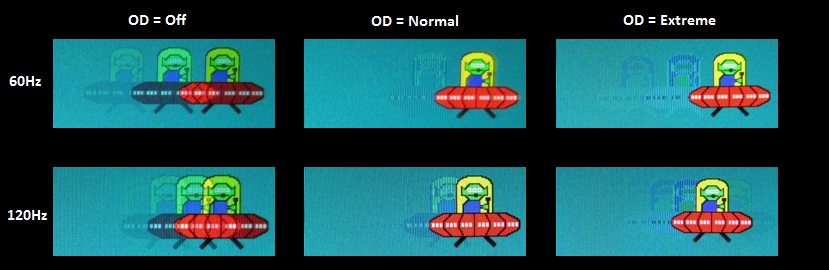
\includegraphics[width=\textwidth]{Chapter04/res/overdrive_ufotest.png}
	\caption{Esempio di artefatti generati dall'overdrive dei pixel (da anandtech.com)}
	\label{fig:overdrive_ufotest}
\end{figure}

Non esiste uno standard per la misurazione dell'overdrive, quindi in questo test vengono proposti due metodi:\begin{itemize}
	\item \texttt{Assoluto}: considera l'errore sull'intero range di luminosità del display. Ad esempio, se durante una transizione da 16 a 32 si raggiunge un livello di 48, l'overshoot è $\frac{48-32}{255}=6.25\%$ . Questo è il metodo consigliato
	\item \texttt{Relativo}: considera l'errore relativo al range di luminosità che la transizione deve percorrere. Ad esempio, se durante una transizione da 16 a 32 si raggiunge un livello di 48, l'overshoot è  $\frac{48-32}{32-16}=50\%$. Questo metodo tende a sovrastimare molto i risultati su transizioni piccole, per cui è quindi generalmente sconsigliato
\end{itemize}

Tra tutti i test implementati nell'applicazione, questo è quello che soffre di più della presenza di rumore, soprattutto retroilluminazione PWM, poiché il test deve misurare delle caratteristiche nel segnale che potrebbero avere una frequenza molto alta. La figura \ref{fig:pixelOverdriveTest_example1} mostra come il segnale potrebbe presentarsi, prima in modo pulito, e poi in presenza di PWM. Si può osseravare fin da subito che se la frequenza della retroilluminazione PWM è troppo bassa, è completamente impossibile ricostruire il segnale originale, per cui in presenza di retroilluminazione PWM il test tende a sottostimare significativamente l'errore.

\begin{figure}[H]
	\centering
	\begin{tikzpicture}
		\begin{axis}[name=Segnale, xmin=0,xmax=0.3,ymin=0,ymax=1023,width=.45\textwidth,xlabel=Tempo (s),ylabel=Valore,xticklabel style={/pgf/number format/fixed}]
			\addplot[black] file{Chapter04/res/pixelOverdriveTest_example_normal.txt};
		\end{axis}
	\end{tikzpicture}
	\begin{tikzpicture}
		\begin{axis}[name=Segnale, xmin=0,xmax=0.3,ymin=0,ymax=1023,width=.45\textwidth,xlabel=Tempo (s),ylabel=Valore,xticklabel style={/pgf/number format/fixed}]
			\addplot[black] file{Chapter04/res/pixelOverdriveTest_example_pwm.txt};
		\end{axis}
	\end{tikzpicture}
	\caption{Segnale senza PWM (sinistra) e segnale con PWM (destra). (Simulato, non è una cattura reale)}
	\label{fig:pixelOverdriveTest_example1}
\end{figure}

Il grafico in figura \ref{fig:pixelOverdriveTest_example2} mostra il segnale ricostruito dall'algoritmo osservando i picchi in presenza di retroilluminazione PWM. Il segnale ricostruito in questo caso ha comunque un picco in corrispondenza dell'overshoot, ma è più piccolo e potrebbe essere addirittura assente, per cui non può essere misurato accuratamente dall'applicazione. Le transizioni dal chiaro allo scuro sono più affette da questo problema rispetto a quelle dallo scuro al chiaro.

\begin{figure}[H]
	\centering
	\begin{tikzpicture}
		\begin{axis}[name=Segnale, xmin=0,xmax=0.5,ymin=0,ymax=1023,width=.7\textwidth,xlabel=Tempo (s),ylabel=Valore,xticklabel style={/pgf/number format/fixed}]
			\addplot[lightgray] file{Chapter04/res/pixelOverdriveTest_example_pwm.txt};
			\addplot[red] file{Chapter04/res/pixelOverdriveTest_example_phf.txt};
		\end{axis}
	\end{tikzpicture}
	\caption{Segnale con PWM (grigio), Segnale filtrato con PeakHoldFilter (rosso). (Simulato, non è una cattura reale)}
	\label{fig:pixelOverdriveTest_example2}
\end{figure}

Il test ha alcuni parametri in input, da passare al costruttore:\begin{itemize}
	\item \texttt{int step}: dimensione del passo tra un livello di luminosità e un altro, sul range 0-255. Si consigliano 16, 32 o 64. Valori più bassi rendono il test più lungo, ma testano più transizioni. (Nota: il valore è espresso nel range 0-255 solo per comodità, internamente vengono convertiti in float nel range 0-1 indipendenti dal formato dei pixel)
	\item \texttt{boolean skipTo0And255}: velocizza il test saltando le transizioni verso 0 e 255, poiché normalmente la luminosità non può scendere sotto il livello di nero, nè sopra il livello di bianco
	\item \texttt{int method}: permette di scegliere tra i due metodi di misurazione (\texttt{METHOD\_ABSOLUTE} o \texttt{METHOD\_RELATIVE})
\end{itemize}

Il seguente pseudocodice mostra il funzionamento del test.
\lstinputlisting{Chapter04/res/PixelOverdriveTest_pseudocode.txt}

Al termine del test, viene chiamato il callback \texttt{onDone} con le seguenti informazioni:\begin{itemize}
	\item \texttt{int[] steps}: array contenente i livelli di luminosità usati nel test come interi nel range 0-255
	\item \texttt{boolean flickeringDetected}: true se il test ha rilevato rumori, come retroilluminazione PWM, che potrebbero ridurre l'accuratezza del test
	\item Molti elementi \texttt{double eFrom>To}: la percentuale di overshoot/undershoot misurata nella transizione da \texttt{From} a \texttt{To}, dove \texttt{From} e \texttt{To} sono elementi dell'array steps. Sono omessi gli elementi in cui \texttt{From=To}, il cui valore è da considerarsi 0
\end{itemize}

\subsection{Input lag (test interattivo)}
La classe \texttt{InteractiveInputLagTest} implementa un test della latenza toatle del sistema, ma a differenza di quello discusso precedentemente, questa è una versione interattiva anziché automatica. A differenza del test automatico, questo test non utilizza affatto un backend grafico: si limita a ricevere i dati dal dispositivo e analizzarli mentre li riceve. Questo test consente di testare il ritardo di input di applicazioni grafiche esterne, in particolar modo videogiochi, in esecuzione sulla stessa macchina o addirittura su una macchina separata.

Il funzionamento del test può essere descritto in modo intuitivo dall'automa a stati finiti in figura \ref{fig:interactiveInputLagTest_fsm}.

\begin{figure}[H]
	\centering
	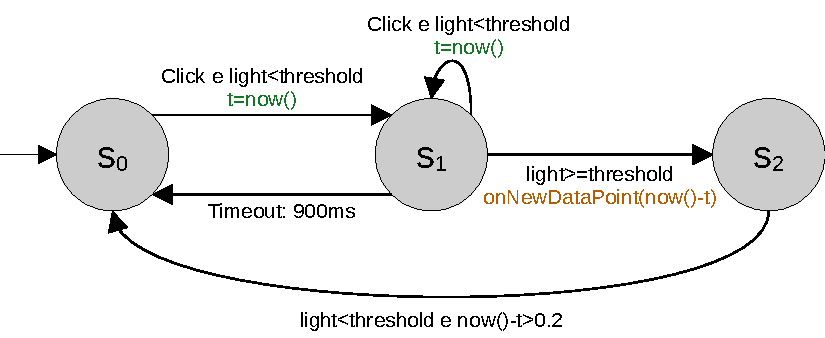
\includegraphics[width=.8\textwidth]{Chapter04/res/interactiveInputLagTest_fsm.pdf}
	\caption{Funzionamento di \texttt{InteractiveInputLagTest}. Le etichette verdi indicano operazioni su variabili, quelle rosse dei callback}
	\label{fig:interactiveInputLagTest_fsm}
\end{figure}

I tre stati hanno i seguenti significati:\begin{itemize}
	\item \textbf{$S_0$}: In attesa del click
	\item \textbf{$S_1$}: Click ricevuto, in attesa del flash
	\item \textbf{$S_2$}: Flash ricevuto, in attesa che finisca
\end{itemize}

All'inizializzazione, è possibile passare al costruttuore due istanze di \texttt{IBuffer}, su cui il test scriverà i valori catturati dal sensore di luminosità e dal pulsante, così che sia possibile visualizzarli nell'interfaccia grafica.

Oltre ai metodi dell'interfaccia standard \texttt{ITest}, questa classe implementa anche i seguenti metodi pubblici: \begin{itemize}
	\item \texttt{public abstract void onNewDataPoint(double delay)}: callback che viene chiamato quando è disponibile un nuovo dato sulla latenza. Il parametro \texttt{delay} contiene il tempo in millisecondi trascorso tra il click e il flash. Attenzione: questo metodo deve terminare il prima possibile per evitare di rallentare il campionamento
	\item \texttt{public void setThreshold(int threshold)}: permette di impostare la soglia di rilevazione del flash come intero tra 0 e 1023
	\item \texttt{public int getThreshold()}: ritorna la soglia di rilevazione del flash corrente come intero tra 0 e 1023. Il valore di default è 100
	\item \texttt{public void setSensitivity(byte sensitivity)}: imposta la sensibilità del sensore tra i quattro valori possibili (0=minima, 3=massima)
	\item \texttt{public byte getSensitivity()}: ritorna la sensibilità attuale del sensore. Il valore di default è 2
	\item \texttt{public void setAutoFire(boolean autoFire)}: permette di attivare o disattivare la generazione automatica dei click anziché utilizzare il pulsante esterno
	\item \texttt{public boolean getAutoFire()}: ritorna \texttt{true} se il dispositivo sta generando i click, false se li riceve dal pulsante esterno. Di default li riceve dall'esterno. Il valore di default è \texttt{false}
	\item \texttt{public byte getState()}: ritorna lo stato attuale dell'automa in figura \ref{fig:interactiveInputLagTest_fsm}
\end{itemize}

Il test prosegue indefinitamente fino a quando non viene terminato manualmente dall'utente chiamando il metodo \texttt{onCancel}. Il callback \texttt{onDone} viene comunque chiamato alla terminazione ma non gli viene passato nessun dato.

Il test può essere utilizzato in due modi:\begin{itemize}
	\item \textbf{Sulla stessa macchina}: in questo caso è sufficiente avviare il test e attivare la generazione automatica dei click. Il dispositivo genera click a una frequenza di circa 1 click al secondo, e posizionando il dispositivo in corrispondenza del muzzle flash di un'arma o qualche altro elemento del gioco che genera un flash in risposta ai click, è possibile misurare quanto tempo passa tra un click e la generazione del flash
	\item \textbf{Su una macchina separata}: si avvia il test utilizzando come fonte dei click il pulsante esterno, si collegano i pin del pulsante esterno ad un mouse o appositamente modificato come spiegato nel capitolo precedente sull'hardware, si posiziona il sensore sul display della macchina da testare come nel caso precedente, e il test misura il tempo che passa tra la pressione del pulsante e la generazione del flash. Si consiglia di far passare almeno mezzo secondo tra un click e l'altro
\end{itemize}

Durante il test, è possibile regolare manualmente la soglia di rilevazione del flash e la sensibilità del sensore. La soglia di rilevazione deve essere impostata il più bassa possibile, ma alta abbastanza da non attivarsi accidentalmente. Per risultati migliori, è consigliabile posizionarsi in un'area scura e utilizzare un'arma o un altro elemento del gioco che genera un flash immediatamente quando viene premuto il pulsante, senza eseguire un'animazione prima.

\subsection{Light to sound}
La classe \texttt{InteractiveLightToSound} implementa un altro test interattivo, che consente di ascoltare il segnale catturato dal dispositivo. Pur non producendo alcun risultato, questo test consente di puntare il dispositivo verso lampadine o altri dispositivi luminosi e sentire immediatamente se la luce è stabile o se ha disturbi. Nel caso delle lampadine, i disturbi sono principalmente causati da un circuito di rettificazione e filtraggio dell'alimentazione inadeguato che causa un flickering a 50 o 100Hz più o meno visibile, che a lungo termine può affaticare la vista.\\
Il test è implementato utilizzando le classi dell'audio \texttt{javax.sound.sampled}. Durante il test, è possibile variare il volume dell'output e la sensibilità del sensore.

Oltre ai metodi dell'interfaccia standard \texttt{ITest}, questa classe implementa anche i seguenti metodi pubblici: \begin{itemize}
	\item \texttt{public void setSensitivity(byte sensitivity)}: imposta la sensibilità del sensore tra i quattro valori possibili (0=minima, 3=massima)
	\item \texttt{public byte getSensitivity()}: ritorna la sensibilità attuale del sensore. Il valore di default è 2
	\item \texttt{public void setVolume(int volume)}: imposta il volume dell'output come un numero tra 0 e 1
	\item \texttt{public float getVolume()}: ritorna il volume corrente. Il valore di default è 1
	\item \texttt{public double getSampleRate()}: ritorna il sample rate in Hz
	\item \texttt{public IBuffer getChartBuffer()}: ritorna un'istanza di \texttt{CircularBuffer} contenente l'ultimo mezzo secondo di audio, così che sia possibile visualizzarlo nell'interfaccia grafica. Il contenuto del buffer ritornato è sempre aggiornato, non è necessario riottenerlo ogni volta che serve
	\item \texttt{public double getStrongestFrequency(double from, double to)}: ritorna la frequenza in Hz più forte nel range specificato, oppure -1 se non ce ne sono o sono troppo deboli per essere rilevanti
\end{itemize}

Il test prosegue indefinitamente fino a quando non viene terminato manualmente dall'utente chiamando il metodo \texttt{onCancel}. Il callback \texttt{onDone} viene comunque chiamato alla terminazione ma non gli viene passato nessun dato.

%RIMOSSO PER DUBBIA UTILITÀ, meglio metterlo nella documentazione
%\subsection{Template per test automatici}
%Il seguente listato mostra il codice minimo per eseguire un test automatico utilizzando i backend grafici forniti e un thread eseguire per il test.
%
%\lstinputlisting[language=Java]{Chapter04/res/TestExample.java}
%
Questo conclude la sezione dedicata all'implementazione dei test.
